\section{Crystal orientation fabric}

Each grain's c-axis is drawn from a Watson distribution about a
chosen mean direction. The user-facing strength parameter is the
leading orientation-tensor eigenvalue $a_1$, the number ice thin
sections actually report: $a_1 = 1/3$ is random, $a_1 = 1$ a perfect
single maximum. The builder converts $a_1$ to the
Watson concentration $\kappa$ internally
(\cmd{kappa\_for\_eigenvalue}), so simulated fabrics are specified in
the same units as the field data they are compared against.

The mean direction is selectable. The default is in-plane, because
the azimuthal method reads the c-axis through second-harmonic
velocity patterns that an in-plane fabric produces directly; a
vertical (disk-normal) fabric is the method's null case and is
available precisely to demonstrate that. A spatial-correlation
control makes neighbouring grains more alike, which lowers boundary
disorientation and therefore scattering, independent of the bulk
fabric strength: bulk anisotropy and local disorder are deliberately
separate knobs, because the first drives the coherent $2\varphi$
velocity signal while the second drives the incoherent scattered
field.

Grain orientations, like the tessellation, are seed-repeatable, and
the realised (not target) orientation tensor is always reported,
since a 100-grain specimen realises the target distribution only
approximately. Figure~\ref{fig:pole} shows the realised fabric of the
title-page specimen on an equal-area pole figure.

\begin{figure}[htb]
  \centering
  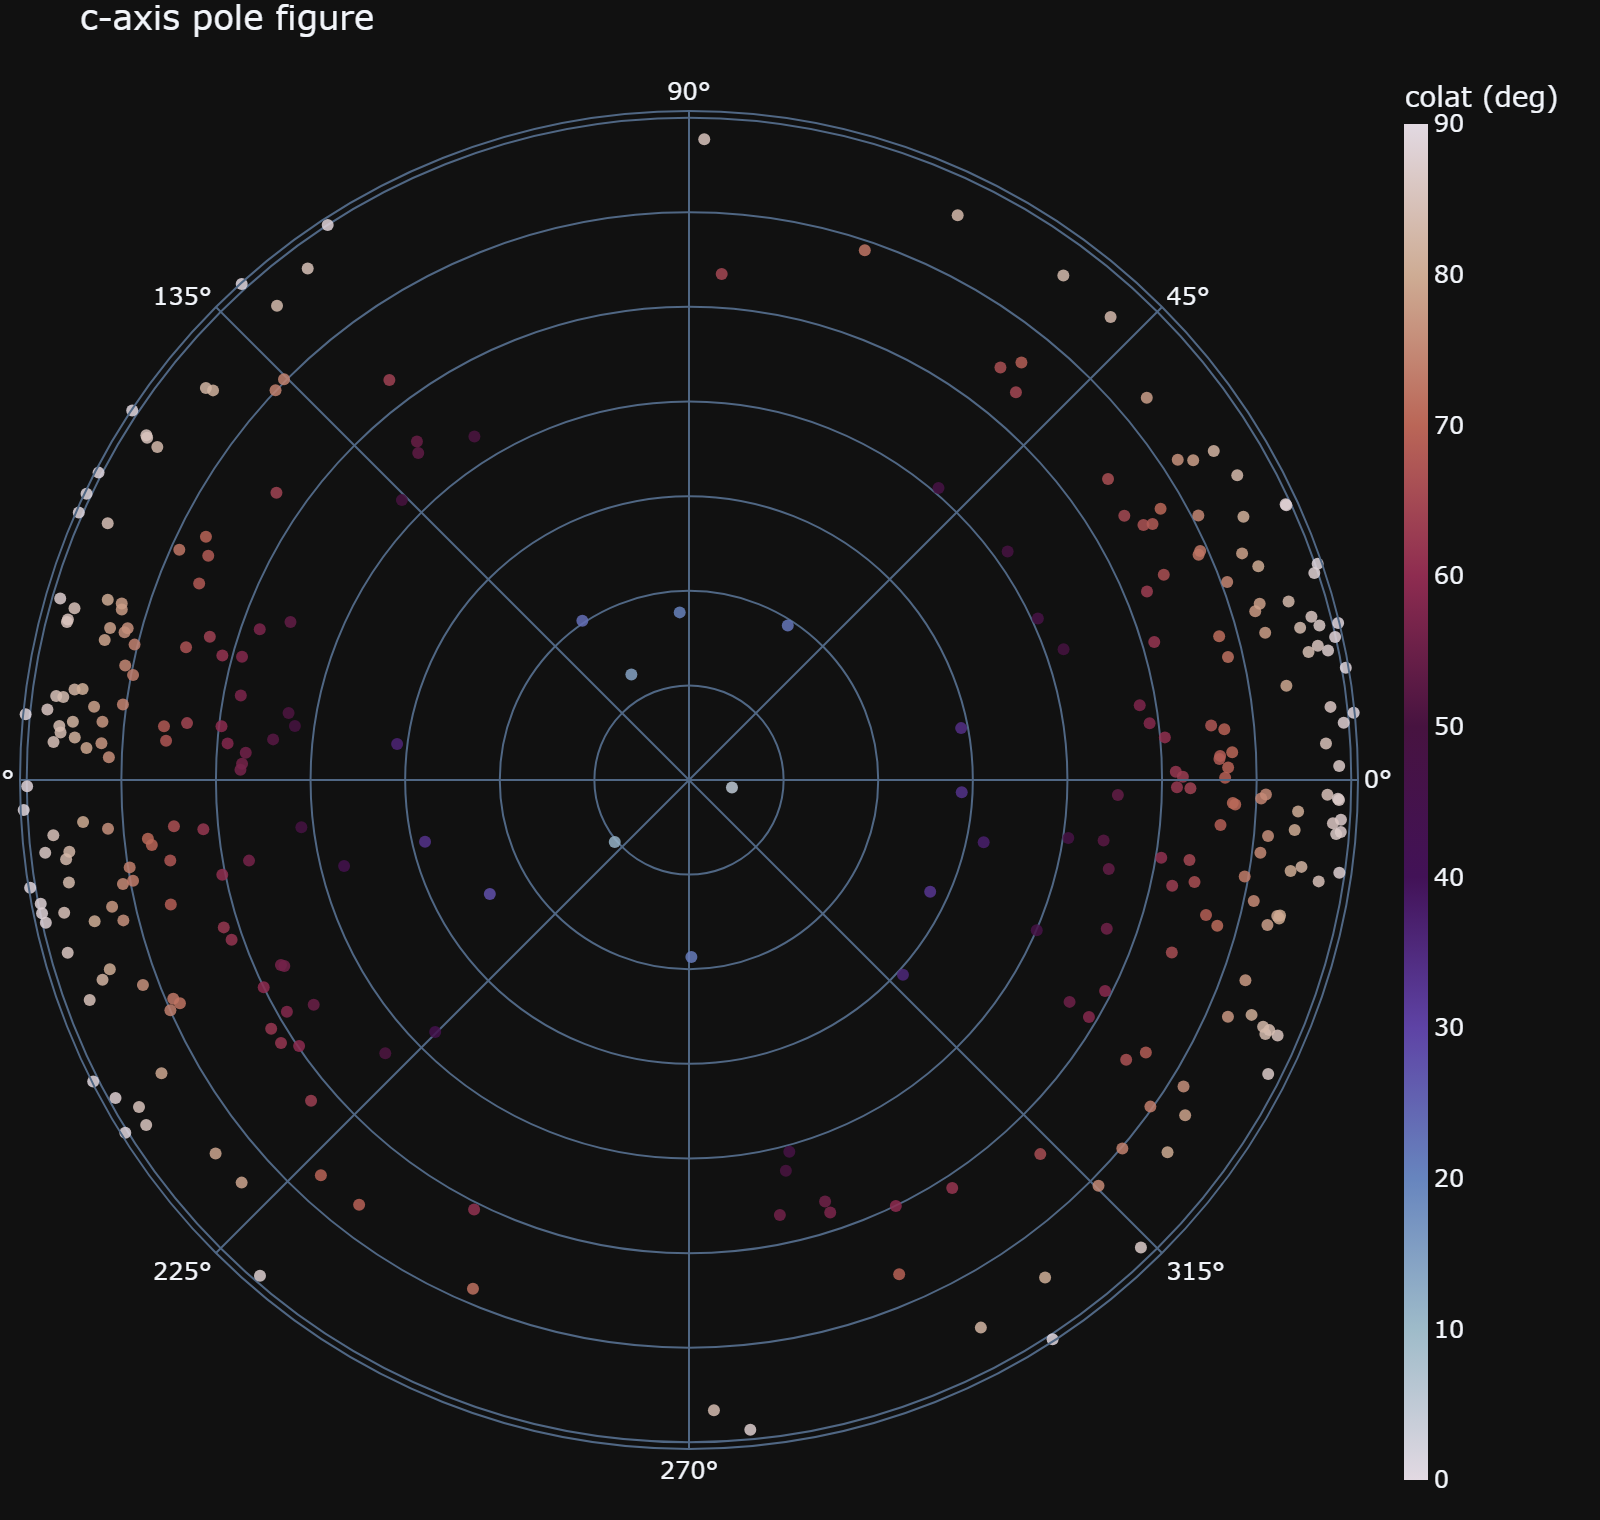
\includegraphics[width=0.55\textwidth]{figures/pole-figure.png}
  \caption{Equal-area (Schmidt) lower-hemisphere pole figure of the
    300-grain specimen at $a_1 = 0.70$ with an in-plane mean c-axis:
    a moderate single-maximum fabric.}
  \label{fig:pole}
\end{figure}
